\section{Course intro and motivation}
\subsection{Terminology}
Information systems: Made of all pieces of data and information used/stored/processed for the needs of the users and applications of enterprises.

Model: Anything used to represent anything else. It can be a physical object, a mathematical or logical representation. Anything. It is more abstract, usually less comprehensive, and cheaper to create that what it models. Important to select which parts to represent as a model. Paper model of some architecture represents the real thing.

Conceptual model: Represents concepts (entities) and relations between them. Information model is a set of informations that represents a model. Information system model represents the system in terms of model. An example of conceptual model. Informations has relations. Represent something from the real world. No costs.

Modelling approach: Non-empty set of semi-formal or formal languages and a number of rules for using these languages to construct models. BPMN has some own rules and syntax.

Enterprise model: Consistent set of special purpose and complementary models describing various facets of an enterprise to satisfy some purpose of some business users. People, processes, services. 

Holistic model: Model that takes into account the differnet aspects or views of the situation or system modelled and how they may affect one another. like functional aspects, performance aspects, user interface aspects etc. Not every aspect or information is valuable for every user.

Model view: Specific aspect of a system or situation that is modelled, like funcitonal views of the system. Contents are viewed from a particular perspective, like contents that a particular user are interested in.

\subsection{Motivation}
Model represents how people perceive an area or a domain. Provides means of common understanding, understand the mechanics that are in play (you may be workign alone). IN large projects, use models if not domain expert to communicate. Important for analysis and requirements, understand what the users want, what they need.


\subsection{Why model}
Several reasons in a variety of sitatuions by variety of model. Model created depends on the reason for modelling. Design model, user model, system image.
We have two perspective: IS and business/enterprise perspective.

IS perspective: To design and develop IT apps. We need to analyse scenarios and user needs for requirements specification. Model is more abstract and maybe cheaper than a program. Provides input to programming processes:
- Requuirements
- Conceptual overview of the app
- Identify modules that can be bought or developed - decision making
- Division of the work according to the capabilties of the app
- Model-driven development - Automation of the dev process.

Business/Enterprise perspective (more important): Look beyond, who is working with waht.
- Analyse and understand a situation: How is the situation perceived by the organization? Obtain an overview of the organization like its organizational structure, functions and resposnbilities. 
- Links IT to organization: IT support for various organizational functions. Design IT to serve organizations. Link IT to business processes.
- Links Business strategy to IT strategy. 
- Develop IT strategy for the organization
- Identifty problems and loopholes
- Design new business processes

\begin{figure}
	\centering
	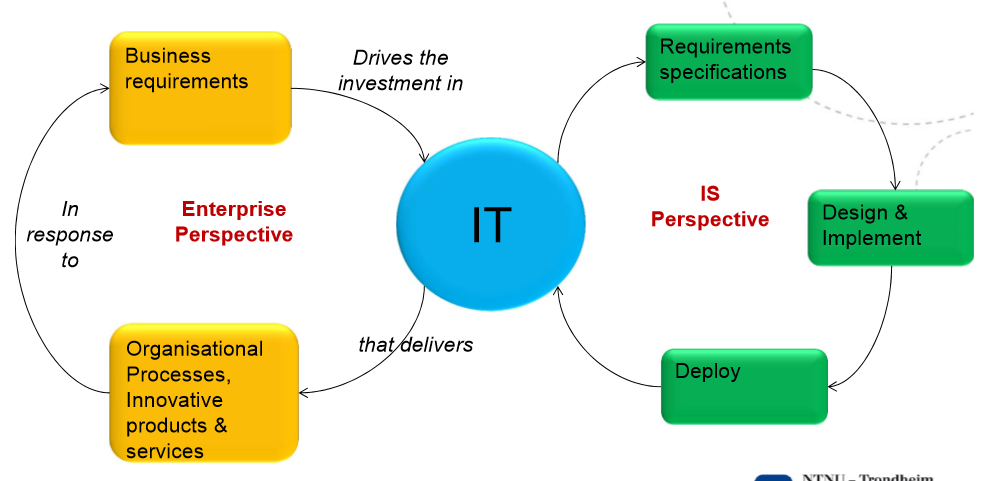
\includegraphics[width=0.8\textwidth]{images/process.png}
	\caption{Model of res}
	\label{fig:whyModel}
\end{figure}

\subsection{Purpose of the Model}
It is important to understand the purpose of modelling and the purpose that would be served by the model that is created. This determines:
- The design and focus of the model
- The perspectives of the model
- The modeling language and approach selected
- The modelling application
- The presentation of the model to the users